\section{Optimal Mechanisms with Both Seller's and Bidder's Cost}

In this section, we take out the constraints and prove that MVAs are optimal in
general. We will also try to find the specific MVA to achieve such optimality,
which turns out to be significantly more complex than previous
simplified case.

The first constraint we are going to remove is seller's cost only.  It's
exciting to introduce bidder's bidding cost since it occurs very often in real
cases and it plays an important role.  Sending emails, making phone calls,
enterring credit card nubmers, depositing money and clicking buttons are all
costly for bidders, though sometimes very tiny.  Bidders may not bid when this
cost is greater than their expected utility. Note that even if the valuation is
very high, the expected utility can be very small because of tense competition,
which is very common on the Internet as $n$, the number of potential bidders,
is very large. 

This behaviour (bidders won't bid because of competitions) is very different
compared to that in previous model [cite Sequential Optimal Auctions] of
sequential auctions. In that model, there's a time discount which
makes bidders eager to bid in early rounds with high reserve prices to avoid
waiting lost. That makes a lot sense in some cases but sometimes it may not.
For example, if the seller posts an auction with a very low reserve price in
the first round, most bidders with high valuation must be happy to bid
according to that time discount cost model. But this may not be true. For
example, when I encounter such an auction online \footnote{For example, when I
see a very good item in the Auction House of Diablo III with a very low current
bidding}, I might be very reluctant to bid because there's a big probability
that my bidding will be over taken by someone else's so it's just a waste of
effort. Our cost model can describe this behaviour very well.

Assume an extreme case where the broadcast cost is $0$, the bidder's bidding
cost is $0.1$ and there are $n \rightarrow \infty$ many $[0, 1)$-uniform
distributed bidders. In a Dutch auction (a Dutch auction has infinite many
rounds of broadcasts so we have to set braodcast cost to $0$), only one bidder
is expected to bid (no competition), thus every bidder with a valuation $v_i
> 0.1$ should be benifitable to bid when the reserve price drops to a little
bit below $v_i-0.1$ (recall that $n \rightarrow \infty$).  In a Vickrey
auction, however, the competition is very tense. Only bidders with valuation
greater than $t$ can accept such intense competition where $t$ satisfies
$t^{n-1}t - 0.1 = 0$ (the expected utility for a bidder with valuation $t$ is
$0$).  Thus $t = \sqrt[n]{0.1}$ which is arbitrary close to $1$ as $n$ grows to
infinity.  Thus almost all bidders can't bare this competition when $n$ is
really large.

So a bad mechanism (e.g. a Vickrey auction) with too much cost will have less
participations and therefore may decreases seller's profit significantly.  To see
this, look at previous extrame case again.  The revenue of Dutch auction will
converge to $0.9$ (someone with valuation very close to $1$ will bid for price
very close to $0.9$) when $n$ becomes infinity.  The revenue of a Vickrey
auction, however, is only $\int_t^1 x \, (n-1) \,n\,( 1-x) \,{x}^{n-2} dx$
which converges to about $0.67$ when $n$ grows to infinity.  

Another problem caused by bidder's cost is that revenue equivalence theorem
seems to be no longer applicable. That's not strange as the revenue equivalence
theorem assumes that the utility of a bidder is equal to the valuation minus
the payment. This assumption is no longer true as now the utility is also
influenced by the cost charged to this bidder.

Finally, because of allowing bidding costs, it seems that we also have to remove
efficiency constraint. Let's consider the case where the highest valuation is
below the bidding cost. Without compensation to bidders, enforcing efficiency means
bidders with highest valuation have to bid (so we can allocate the item to
them) which would make their expected utility negative.

In summary, we now introduce bidder's bidding cost and drops efficiency
constraint for our mechanisms. The first issue we are going to solve is to make
revenue equivalence theorem, or a very similar theorem, applicable to our model
again. 

\subsection{Spending Equivalence Theorem and Revenue Optimization Strategy}

\begin{theorem}\label{theorem:equivalence}

The expected overall spendings from all bidders (including their bidding costs
and payments to the seller) in a feasible mechanism (with our cost model) is
completely determined by the expected utility of lowest type bidders and
allocation probability function
$$p: (v_1, v_2, \ldots, v_n) \rightarrow (p_1, p_2, \ldots, p_n)$$ 
where $p_i$ is the probability that bidder $i$ will get the item.

\end{theorem}

\begin{proof}
This theorem is exactly the same as revenue equivalence theorem except that we
exchange revenue with spending. To prove it, let's construct another mechanism
$M'$ without bidding cost from our mechanism $M$ with bidding cost so $M'$ fits
into the original revenue equivalence theorem's model. Suppose there's a
virtual seller in $M'$, who collects valuations from all bidders at no cost (a
direct revelation mechanism). Then this virtual seller will make $n$ virtual
bidders delegating bidders to communicate with the true seller in our mechanism
$M$.  When our mechanism ends by allocating the item to virtual bidder $i$, the
virtual seller also allocate the item to the real bidder $i$. The payment from
each bidder $i$ to this virtual seller will be equal to the payment that
virtual bidder $i$ pays to our real seller plus all the bidding costs charged
to virtual bidder $i$. Thus, from the real bidders' aspects, this mechanism
$M'$ is just a direct revelation mechanism which will satisfy revenue
equivalence theorem. The only difference is that the payment from real bidder
$i$ to the virtual seller actually has two parts, one is payed to the real
seller, another is payed to bidding costs, which sum up to the total spending.
\end{proof}

Thanks to theorem \ref{theorem:equivalence}, our profit maximization problem
is now greatly simplified: 

\begin{corollary}
To maximize profit for a given allocation rule $p: (v_1, v_2, \ldots, v_n)
\rightarrow (p_1, p_2, \ldots, p_n)$, we only need find the minimum total cost
(including both seller's cost and bidders' cost).
\end{corollary}

\begin{proof}
The total spending, substracts cost charged to bidders, will be the revenue
that the seller receives.  This revenue, substracts cost charged to the seller,
will be profit. Thus profit is total spending minus total cost. As total
spending is fixed by allocation rule, we only need to find the minimum cost to
maximze profit.
\end{proof}

The highlight here is that we won't have to differentiate cost charged to
bidders and cost charged to sellers if we just want to maximize seller's profit.
The difference of them may make revenue different, but as long as their sum
doesn't change, the profit won't change. This not only helps us simplify our
analysis, but also helps us simplify the optimal mechanism: the seller could
just design a mechanism with compensations to help bidders pay all the bidding
cost. Thus the bidders won't bother the cost.

There's one more challenge, however: the optimal allocation rule here
isn't as simple as the one that's discovered by Myerson [ref:Optimal Auction]:
allocate the item to the bidder with highest virtural value if it's positive.
This rule, though optimal in Myerson's setting, may not be optimal here. Theorem
\ref{theorem:equivalence} tells us that this rule will maximize the total spending.
But we must substract the cost from the spending to get the profit. Therefore,
there might be another weird allocation rule that has less total spending but even
much less minimum cost.

It's not hard to find one example of this. We know that for bidders
with uniform valuation over $[0, 1)$, the spending maximizing allocation rule
is allocate the item to the bidder with highest valuation that's greater than $1/2$.
However, if the broadcast cost is too large, for example $1$ (which is equal to the
highest possible valuation), the cost to find out whether there's any bidder with valuation
greater than $1/2$ is at least $1$. Thus if we use this allocation rule, the
final profit would be negative since the total spending must be less than the
minimum cost. However, the allocation rule that never allocate the item will have
$0$ cost and $0$ spending, which achieves $0$ profit, better than previous allocation
rule.

Thus, the revenue optimal mechianism will depend on how minimum cost is defined. 
We previously defined how cost is charged and proved that a specific mechanism (MVA)
has minimum cost when allocation rule is allocate efficiently. But unfortunately,
that's not enough to give us a well defined minimum cost for any allocation rule.
For example, one allocation rule might be always allocate the item to each bidder
with the same probability $1/n$, i.e. $p(v_1, v_2, \ldots) = (1/n, 1/n, \ldots)$.
You might think that the minimum cost for this is $0$ since we don't have to know
anyone's valuation. But that cost isn't realistic: how can you ever allocate the
item to someone that you have never communicated with? Thus the minimum cost seems
to be at least $b$, the cost for one round of broadcast, if we ever allocate the item
to some bidder. In order to make a realistic constraint and get a well defined minimum
cost for any allocation rule, we define

\begin{definition}\label{def:allocation_cost}
For an allocation rule $$p: (v_1, v_2, \ldots, v_n) \rightarrow (p_1, p_2,
\ldots, p_n)$$ if $p_i > 0$ for some valuation profile $(v_1, v_2, \ldots,
v_n)$, there must be a broadcast query that the $i$-th bidder with valuation
$v_i$ reply to the seller under that profile setting.
\end{definition}

With this definition, we have

\begin{theorem}
The optimal mechanism should always allocate the item to the bidder with
highest virtual valuation $v_i - \frac{1-F(v_i)}{f(v_i)}$ if it decides to
allocate the item. In regular cases when the virtual valuation is monotone
strictly increasing, the optimal mechanism should always allocate the item to
the bidder with highest valuation if it decides to allocate the item.
\end{theorem}

To see why this theorem holds, firstly notice that in our cost model, the
minimum cost to let any bidder reply is equal to the minimum cost to let the
max-valuation bidder or max-virtual-valuation bidder to reply.
This is because that the mechanism is only allowed to ask broadcast
queries and it's equivalent to specify a range $Q \subseteq [0, 1)$ and ask all
bidders whose valuations are within that range to reply. That means, by
properly mappings of valuations and query ranges, we can always adapt a
strategy that lets any bidder reply to another strategy that lets the
max-virtual-valuation bidder reply and vise versa (just like what we did to prove lemma
\ref{lemma:descending}). This means that finding the max-valuation bidder won't
cost more than any other cases except doing nothing (which costs $0$). Thus the
optimal mechanism either do nothing (no one replies and thus $p_i = 0$ by
definition \ref{def:allocation_cost}) which has minimum cost or ask queries to
find the max-virtual-valuation bidder and allocate the item to that bidder which has
maximum total spending.  The flexibility of an optimal mechanism is that it can
choose the cases in which it won't allocate the item (in any other cases it
will allocate the item to the max-virtual-valuation bidder). It's also intuitive
to see that the no allocation cases can be described by a single parameter $l$:
no allocation if every bidder's valuation is below $l$. For limit of space,
we won't list the detailed proof for the above theorem and arguments.

For simplicity, we won't mention virtual valuation below because they are 
indifferent in terms of minimizing cost.  For convenience, we will use
valuation instead of virtual valuation even if we are later talking about
profit because our mechanism are just going to find the maximum value and it's
equivalent to finding the maximum virtual value in regular cases.

Now we can narrow our optimal mechanisms with relaxed efficiency constraint:

\begin{definition}

We say mechanisms satisfy relaxed efficiency constraint with low value $l$
if:

    \begin{enumerate}

    \item They only allocate the item to bidders whose valuation are at least
    $l$ (the low value is $l$)

    \item If they will allocate the item, they will always allocate the item to
    the bidder with highest valuation.

    \end{enumerate}

When we say a mechanism has a low value $l$, we imply that this mechanism
satisfy relatex efficiency constraint with low value $l$.

\end{definition}

\subsection{MVAs' Optimality in General}

We have already narrowed down optimal mechanism to
relaxed efficient mechanisms and by theorem \ref{theorem:equivalence},
it's straightforward to see

\begin{corollary}

For mechanisms with a fixed low value $l$, the maximum profit is
achieved when the mechanism minizes the cost.

\end{corollary}

Our next question is naturally: what's the cost minimized mechanism
given a low value $l$. As expected:

\begin{theorem}

MVAs have the minimum cost among all mechanisms with a low value $l$

\end{theorem}

\begin{proof}
A special case of this theorem when $l = 0$ is theorem \ref{theorem:MVA_eq}.
We proved that special case by introducing lemma \ref{lemma:uniform} and
\ref{lemma:descending}. To prove the general cases with arbitrary $l$, we just
need to revise lemma \ref{lemma:uniform} a little as following lemma
\ref{lemma:lowest_type}. All other part of the proof remains similar. For space
limit, the detailed proof is omitted.
\end{proof}

\begin{lemma}\label{lemma:lowest_type}
Suppose that there are two cases $n, F_1, f_1, l_1$ and $n, F_2, f_2, l_2$
where $n$ is the number of values for both cases, $F_i, f_i$ are CDF and PDF
of the $n$ i.i.d. values in case $i$, $l_i$ is the low value for case $i$.
If $F_1(l_1) = F_2(l_2)$, then these two cases have the same minimum cost
to find the maximum value above the low value $l_i$.
\end{lemma}

The proof of this revised lemma is almost identical to the one for original
lemma. Thus for space limit, we won't elaborate it again. Finally, we conclude
that MVAs are optimal in general.

\begin{corollary}

MVAs are optimal. The only parameters we are going to determine for the
specific optimal MVA are 1) the low value $l$; 2) the descending query
thresholds $a_1, a_2, a_3, \ldots$.

\end{corollary}

When we later investigate such parameters that minimizes the cost, we will
also assume uniform distribution $F(x) = x$ in default because distribution won't
change this minimum cost and we can always adapt an optimal MVA for uniform distribution
to an optimal MVA for any distribution easily.

\subsection{Experiments to Discover Optimal MVA with a Given Low Value}

To discover the specific MVA that's optimal, we first try to identify the
optimal thresholds $a_i$ given a low value $l$  (recall that in $i$-th round,
MVA will ask all bidders whose valuation is within $[a_i, a_{i-1})$ to bid).
If we can write the minimum cost $C^*$ as a function of $n, \rho, l$ (recall
that $\rho = b/c$ is the ratio between broadcast and bidding cost), we may then
determine the optimal $l$ using this function.

In the special case that we studied in previous section where $l = 0$
(efficiency is enforced), the optimal thresholds can be easily described as a
single parameter $\alpha$. This strategy won't work when $l > 0$ (we assume uniform
distribution in default). Obviously that $a_i \geq l$,
thus we can't let $a_i = \alpha a_{i-1}$ since $\lim_{i \rightarrow \infty} a_i
= 0 < l$.  Additionally, if we revise the equation by letting $a_i-l = \alpha
(a_{i-1}-l)$, we will get a positive possibility $F(l)$ that we would ask
infinite many broadcast queries, which is even worse.

As it's not immediately clear what optimal thresholds should be like, we
present a simple algorithm to calculate such thresholds numerically. We firstly
discretize the continuous valuation $[0, 1)$ to $D$ discrete values $\{0, 1, \ldots,
D-1\}$. That means, the original valuation $v$ will be transformed to integer
value $\hat v = \lfloor v D \rfloor$. Then we use dynamic programming to
inductively calculate $\hat x_{\hat h}$, the length of next optimal descending
query $[\hat h-\hat x_{\hat h}, \hat h)$ to ask, conditional on that we have
already queried $[\hat h, D)$ and no one replies.

\begin{algorithm}
    \caption{Calculate discretized best query lengths}\label{algo:discrete}
    \begin{algorithmic}[1]
        \Require{$\hat l$ is the discretized low value, $\rho$ is the ratio between broadcast and bidding cost,
        $n$ is the number of bidders, $D$ is the maximum discretized valuation}
        
        \Function{BestQueryLengths}{$\hat l$, $\rho$, $n$, $D$}
            \State $\hat x_{\hat l} \gets 0$
            \State $C_{\hat l} \gets 0$
            \For{$\hat h={\hat l}+1 \mbox{ to } D$}
                \State $\hat x_{\hat h} \gets \displaystyle
                  \operatorname*{arg\,min}_{1 \leq \hat x \leq \hat h-l} \rho + n
                  \frac{\hat x}{\hat h} + (\frac{\hat h-x}{\hat h})^n C_{\hat h-\hat x}$
                \State $C_{\hat h} \gets \rho + n \frac{\hat x_{\hat h}}{\hat h} +
                  (\frac{\hat h-\hat x_{\hat h}}{\hat h})^n C_{\hat h-\hat x_{\hat h}}$
            \EndFor
            \State \Return $\hat x$
        \EndFunction
    \end{algorithmic}
\end{algorithm}

Algorithm \ref{algo:discrete} runs in time $O(D^2)$. Having $\hat x$, we can
then infer the best strategy $x$ for original continuous problem by converting
$\hat h, \hat x$ back to $h, x$ and using them to interpolate continuous
strategy.  The larger $D$ is the more accurate it will be. But it will also
require more running time.  Running this for case $l = .5, \rho = 2, n = 10, D
= 1000$ we get $x$ showed in figure \ref{fig:x-h}. It seems that $x$ is a
piecewise linear function over $h$.  For those $h$ which is close to
$l$, obviously that the optimal strategy should be $x = h - l$,
which means using only one query to explore all potential bidders. But it's
unclear why $x$ is linear when the best strategy is using multiple queries to
explore the valuation range.

\begin{figure}
\centering
    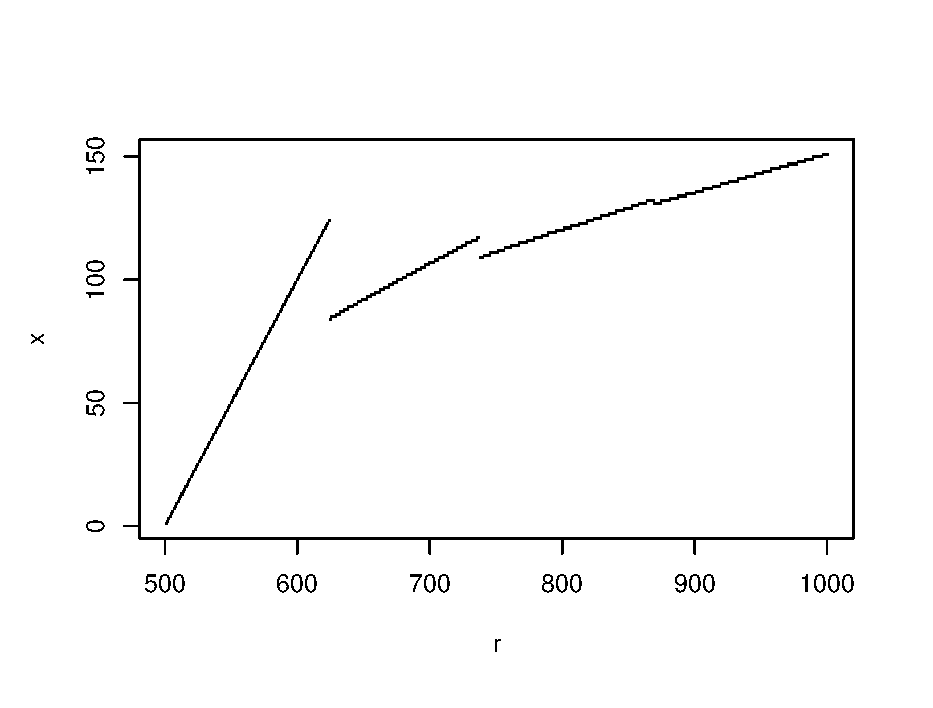
\includegraphics[trim=0mm 5mm 5mm 15mm, clip, width=\linewidth]{figures/1000-500-2-1-10}
    \caption{The best query lengths over $h$ (the highest
        undiscovered value) when discretized low value $\hat l = 500$,
        ratio between broadcast and bidding cost $\rho = 2$,
        number of bidders $n = 10$ and maximum discretized valuation
        $D = 1000$}\label{fig:x-h}
\end{figure}

Another way to plot the graph is to normalize $x$ and $l$ so that $h$ becomes
$1$ since our model is $v_i \in [0, 1)$. It's showed in figure \ref{fig:x-l}.
This again looks like a piecewise linear function.  A more interesting
observation is that the left-most piece is quite a long straight line $x =
1-\alpha$. Thus it seems that $x = 1-\alpha$ is optimal for quite a lot $l$ which is not
far from $0$. Here the $\alpha$ is the the optimal $\alpha$ of $\alpha$-MVA if
we set $l = 0$.

\begin{figure}
\centering
    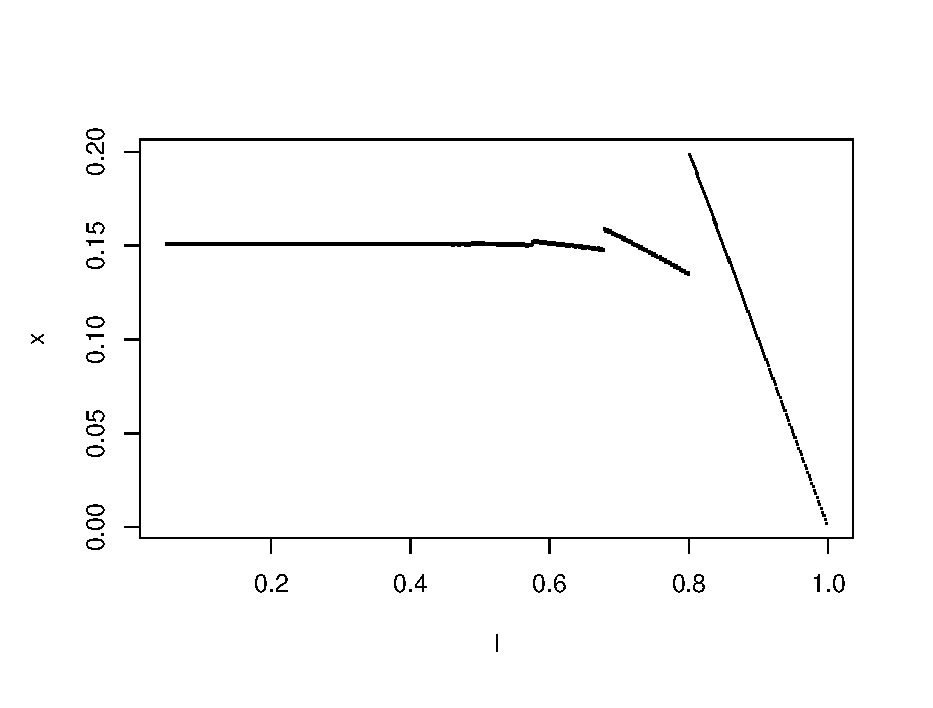
\includegraphics[trim=0mm 5mm 5mm 15mm, clip, width=\linewidth]{figures/10000-500-2-1-10}
    \caption{The normalized best query length $x = \hat x_{\hat h} / \hat h$
    over normalized $l = \hat l / \hat h$ when discretized low value $\hat l =
    500$, ratio between broadcast and bidding cost $\rho = 2$, number of
    bidders $n = 10$ and maximum discretized valuation $D =
    10000$}\label{fig:x-l}
\end{figure}

\subsection{Analysis of Optimal MVA with a Given Low Value}\label{sec:general_analysis}

Figure \ref{fig:x-h} shows that the optimal MVA with a low value $l$ is
much more complicated but there might still be hope to get a nice analytical
result: piecewise linear function. That is, we can't use a single $\alpha$ to
describe such optimal MVA, but perhaps we can use a sequence of $\alpha$ to
describe it. Now let's take an analytical treatment.

The first key to analyze the optimal MVA with low value is to utilize
the fact that there's a fixed maximal number of rounds to exploit the whole
reportable valuation range $[l, h)$ ($h$ is the highest undiscovered
value as defined in last subsection and $h = 1$ initially). Let's call that
number $k$.\footnote{We have argued this before: if such $k$ doesn't exist, or equivalently
the maximum number of rounds is unbounded, the cost will be infinite as the possibility that no
values lie in $[l, h)$ is positive.}

For convenience, define $\vec a = (a_0, a_1, a_2, \ldots, a_k)$, the vector of
$k$ thresholds in such optimal MVA. We make $a_0 = h, a_k = l$ so in $i$-th
round the query would be $[a_i, a_{i-1})$. Now define cost $C(\vec a, k, \rho,
n)$ to be the expected cost for MVA defined by $k, \vec a$ when there are $n$
i.i.d.  $[0, 1)$-uniform bidders (note that $l, h$ are implicitly defined by
$a_k, a_0$). If we can get a neat form of $C$, we can use $\frac{\partial
C}{\partial a_i} = 0 $ to characterize optimal MVA, as we did in section
\ref{sec:alpha-MVA}.\footnote{It's easy to see that boundary cases $a_i = a_{i-1},
a_{i+1}$ are not optimal too.}

Thus the second key is to represent this $C$. Rather than
considering one round after another recursively as we did before, we now consider all
rounds together:
\begin{align*}
C(\vec a, k, \rho, n) =
&\sum_{i=0}^k P\big(H_i = 1\big) C\big(\vec a, k, \rho, n ~\big|~ H_i = 1 \big)
\end{align*}
where $H_k$ is the indicate random variable for the event that the highest
valuation is below $a_k$ and $H_i(0 \leq i < k)$ is for the event that the highest
valuation is in $[a_{i+1}, a_i)$.

Since bidders are uniformly distributed,
\begin{align*}
  &P(H_k = 1) = a_k^n / a_0^n\\
    &P(H_i = 1) = (a_{i}^n-a_{i+1}^n) / a_0^n
\end{align*}

It's also clear that $C(\vec a, k, \rho, n ~\big|~ H_k = 1) = k\rho$ because
there will be only $k$ broadcasts and no biddings.

For $C\big(\vec a, k, \rho, n ~\big|~ H_i = 1\big)$ where $i < k$, we partition
it into two parts $C\big(\vec a, k, \rho, n ~\big|~ H_i = 1\big) = C_b\big(\vec
a, k, \rho, n ~\big|~ H_i = 1\big) + C_c\big(\vec a, k, \rho, n ~\big|~ H_i =
1\big)$. The broadcast part $C_b\big(\vec a, k, \rho, n ~\big|~ H_i = 1 \big)$
is simply $(i+1)\rho$ as the MVA finishes in $(i+1)$-th round. The
not-so-obvious part is the overall bidding cost $C_c\big(\vec a, k, \rho, n
~\big|~ H_i = 1 \big)$. It can be expressed as:

\begin{align*}
P(H_i = 1)C_c\big(\vec a, k, \rho, n ~\big|~ H_i = 1 \big) = E\left( H_i \cdot
    \sum_{j=1}^n X_{ij}\right) \\
= E\left( \left( \prod_{j=1}^n B_{ij} \right) \cdot \left(\sum_{j=1}^n X_{ij}
    \right) \right)
\end{align*}

Here $X_{ij}, A_{ij}$ are both indicate random variables of bidder $j$'s valuation $v_j$:
$$
X_{ij} = \begin{cases}
    0, &\mbox{if $v_j \notin [a_{i+1}, a_{i})$ } \\\\
    1, &\mbox{if $v_j \in [a_{i+1}, a_{i})$}
\end{cases}
~~
B_{ij} = \begin{cases}
    0, &\mbox{if $v_j \geq a_{i}$ } \\\\
    1, &\mbox{if $v_j < a_{i}$}
\end{cases}
$$

You may notice that our original random variable $H_i$ is not exactly the same
as our substitute $\prod_{j=1}^n B_{ij}$. The only difference between them,
however, is the case that every $v_j$ is below $a_{i+1}$, which is the case
that every $X_{ij} = 0$, so the equation still holds.

Now we use the properties of expectation to finish our calculation:
\begin{align*}
  &E\left( \left( \prod_{j=1}^n B_{ij} \right) \cdot \left(\sum_{j=1}^n X_{ij}
  \right) \right) = \sum_{j=1}^n E\left( X_{ij} \prod_{k=1}^nB_{ik} \right)
  \\
    &~~ = \sum_{j=1}^n \left( E(X_{ij} B_{ij}) \prod_{k \neq j} E(B_{ik})
    \right)
       = n a_{i}^{n-1} (a_{i}-a_{i+1}) / a_0^n
\end{align*}
Combine all those above, finally we get (note that low value $l = a_k$ and
$\frac{\partial C}{\partial a_i}$ is only for $1 \leq i \leq k-1$ since
$a_0, a_k$ are constants):
\begin{align}
& C(\vec a, k, \rho, n) = k \rho a_k^n / a_0^n + \nonumber\\ 
    &~~~ \frac{1}{a_0^n} \sum_{i=0}^{k-1} \left( (a_{i}^n-a_{i+1}^n) (i+1)
    \rho + n a_{i}^{n-1} (a_{i}-a_{i+1}) \right) \label{eq:C_general} \\
    &~= \sum_{i=0}^{k-1} \frac{a_i^n}{a_0^n} \left( \rho + \frac{a_i-a_{i+1}}{a_{i}} n \right)
    \label{eq:C_general_simplified}\\
& \frac{\partial C}{\partial a_i} = \frac{1}{a_0^n} \left[
	n(n+\rho)a_i^{n-1}-n(n-1)a_{i+1}a_i^{n-2}-n a_{i-1}^{n-1} \right]
	\label{eq:diff_C_general}
\end{align}

Equation \ref{eq:C_general_simplified} gives another explanation about the
cost: the sum of expected cost of each round. Unfortunately, equation
\ref{eq:diff_C_general} isn't neat enough to get a piecewise linear $a_1$.
Recall that in previous subsection, the experiment seems to show that $x$ is
piecewise linear over $h$, which means $a_1 = a_0-x = h-x$ must also be
piecewise linear over $a_0 = h$.  For example, for the simple case $k = 2, n =
3$, we have: $a_1 =
\frac{\sqrt{{a_0}^{2}\,\rho+{a_2}^{2}+3\,{a_0}^{2}}+a_2}{\rho+3}$.  Anyway, by
definition we have $a_1 \geq a_2$. And
$a_1=\frac{\sqrt{{a_0}^{2}\,\rho+{a_2}^{2}+3\,{a_0}^{2}}+a_2}{\rho+3}$ indeed
looks very linear when $a_1 \geq a_2$.

Though we failed characterizing the optimal MVA using piecewise linear
descriptions, equation \ref{eq:C_general_simplified} gives us a better way to
calculate thresholds $a_i$. Here we use an R package called BB [cite BB] to
solve these non-linear equation systems. Before throw those equations to that
package, we have to first decide $k$ and an initial guess of $a_i$.  One
obvious upper upbound of optimal $k$ is $k_\alpha = \left\lceil \log_{\alpha}
\left(\frac{a_k}{a_0}\right) \right\rceil$ where $\alpha$ is the optimal
$\alpha$ for $\alpha$-MVA when $l = 0$.  (This upper bound seems to be
$\Theta(n)$). We believe that $C$ has a single peak over $k$ (proof?), thus we
can search $k$ efficiently.

The initial $a_i$ is very important for solving optimal $a_i$. A bad choice may
lead to much more computation and even non-convergence. For example, the
trivial uniform $a_i = a_0 - \frac{i}{k}(a_0-a_k)$ is a bad initial guess. We
find the intial $a_i = \alpha^i$ provided by $\alpha$-MVA to be very efficient.
Let's call this $MVA$ with thresholds $\alpha, \alpha^1, \ldots, \alpha^{k-1}$
where $\alpha^{k-1} \geq l, \alpha^k < l$ an $\alpha$-cutoff-MVA, as we did in
previous section \ref{sec:eff_experiment}.  It's suggested by experiments
showed in figure \ref{fig:x-l} where $x$ seems to be $1-\alpha$ for a lot of
$l$. In experiments, the actual optimal $k$ is very close to our upper bound
$k_\alpha$: it's mostly either $k_\alpha$ or $k_\alpha-1$.  This might be a
direct consequence of $\alpha$-cutoff-MVA's good performance shown in figure
\ref{fig:cutoff}. As you can see, in most cases their profit are very close.
The significant difference only occur when low value $l$ is a little below
$\alpha$ and this isn't likely to occur when $n$ is large where $\alpha$ is
much closer to $1$ than $l$.

\begin{figure}
\centering
    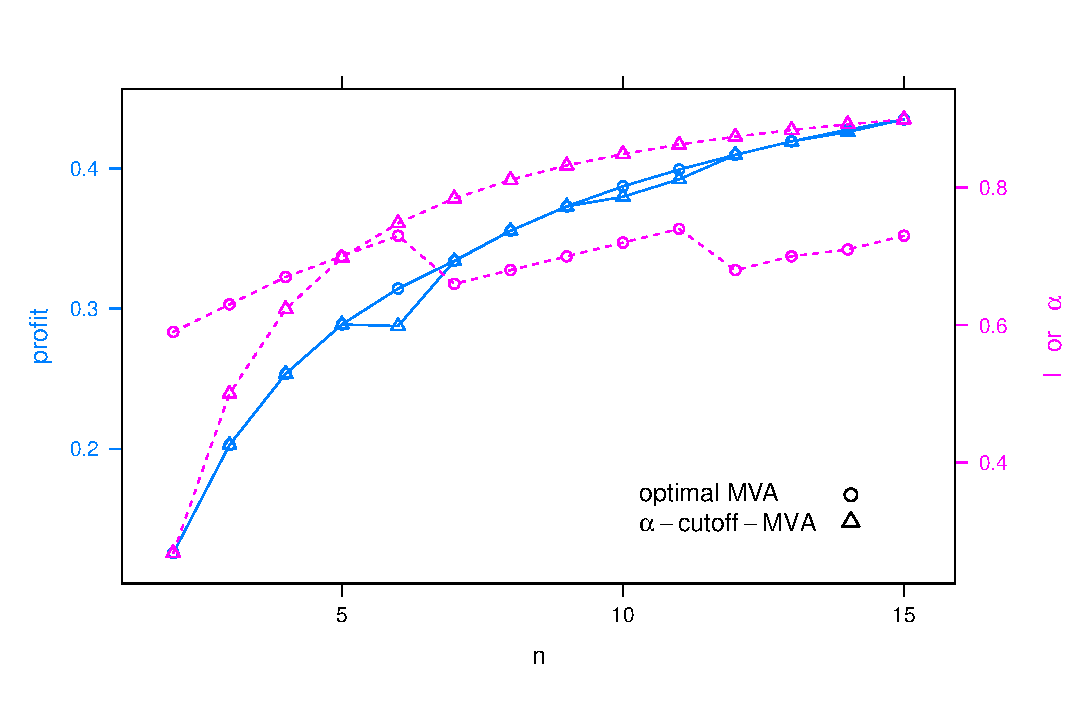
\includegraphics[width=\linewidth]{figures/cutoff_.2_.1_15.eps}
    \caption{The profit of optimal MVA and $\alpha$-cutoff-MVA are plotted in
    solid line.  The low value $l$ is chosen to maximze optimal MVA's profit.
    We also plot $l$ and $\alpha$ in dashed lines to see how they affect the
    relative profit difference.  Note that $\alpha$ does not depend on
    $l$.}\label{fig:cutoff}
\end{figure}

\subsection{Choosing Low Value}

Having $k$ and $a_i$, we are still one step from optimal MVA, choosing the low
value $l$. It's obvious to see that optimal cost $C$ is non-increasing as $l$
increases. By Myerson's optimal auction theory and theorem
\ref{theorem:equivalence}, setting virtual value of $l$ to be $0$ will yield
the maximum total spending. Name such $l$ as $l_0$. We then conclude that
optimal $l$ must satisfy $l \geq l_0$ as the optimal is non-increasing. The
question is, how to search or determine optimal $l$? Let's first check the simple
case when the value distribution is uniform.

Figure \ref{fig:CSP-l-2-1} and \ref{fig:CSP-l-5-1} plot cost, spending and profit
over $l$. It's clear in figure \ref{fig:CSP-l-5-1} that increasing $l$ from $0.5$ to about $0.8$
will get a significant profit increase. However, it's not so clear in these two plots
whether profit is unimodal. To see it more clear, we plot figure \ref{fig:suboptimality},
which transforms the cost, spending and profit to their corresponding suboptimality, i.e.
the distance between the specific value and the optimal value (to make the log-scale work
for distance $0$, we add some small constant to that suboptimality). Thus, the new plot will
preserve the peaks and global optimal point as the lowest point.

\begin{figure}
\centering
    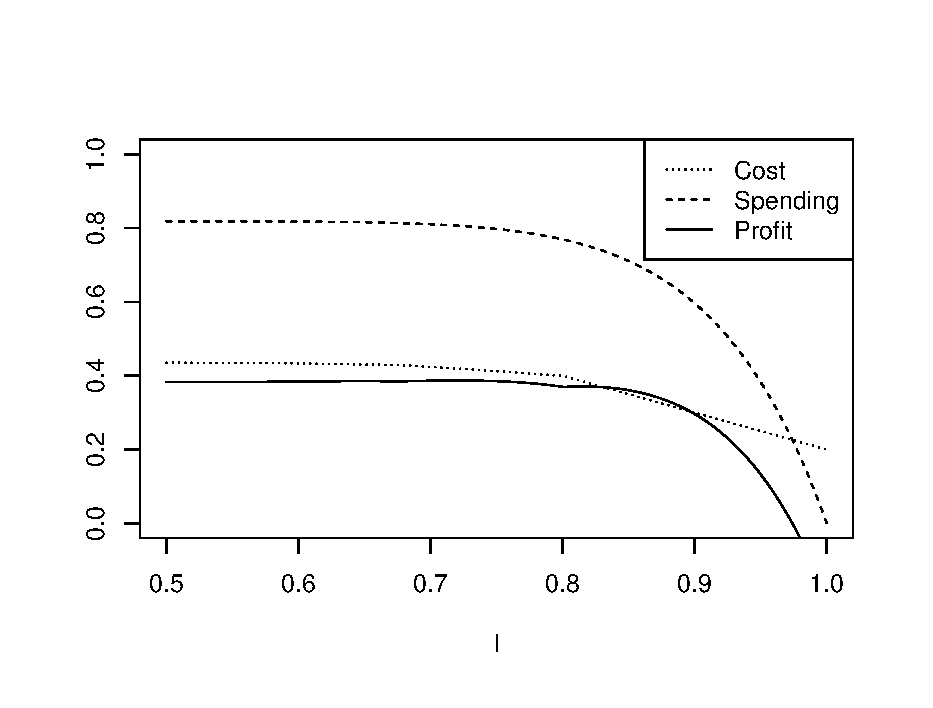
\includegraphics[trim=0mm 5mm 5mm 15mm, clip, width=\linewidth]{figures/10-0.200000-0.100000.eps}
    \caption{Cost, Spending and Profit over $l$ when $n = 10, b = 0.2, c = 0.1$}\label{fig:CSP-l-2-1}
\end{figure}

\begin{figure}
\centering
    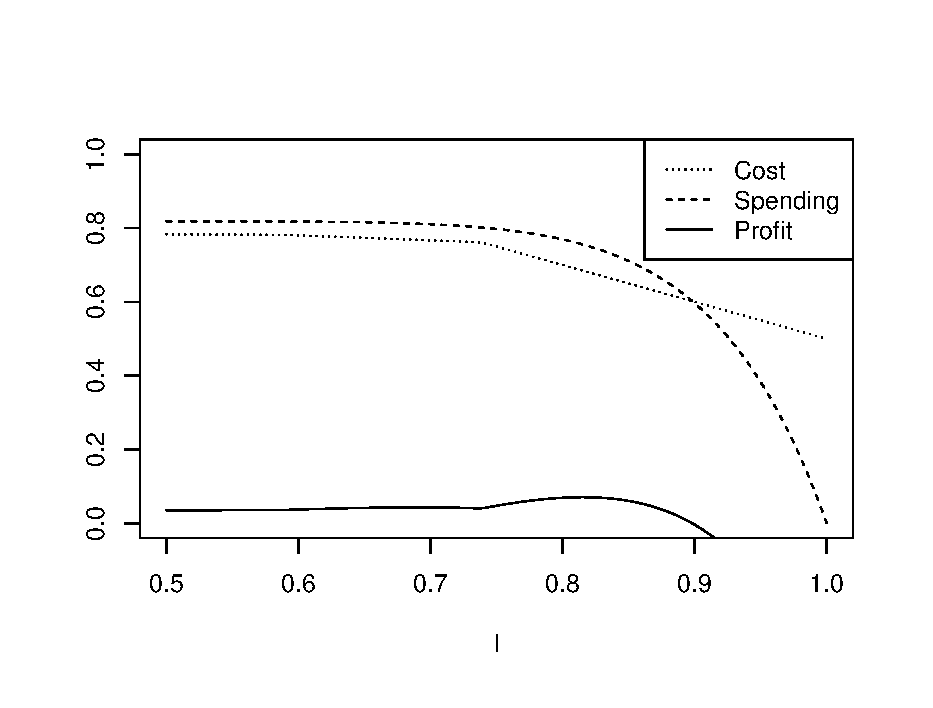
\includegraphics[trim=0mm 5mm 5mm 15mm, clip, width=\linewidth]{figures/10-0.500000-0.100000.eps}
    \caption{Cost, Spending and Profit over $l$ when $n = 10, b = 0.5, c = 0.1$}\label{fig:CSP-l-5-1}
\end{figure}

\begin{figure}
\centering
    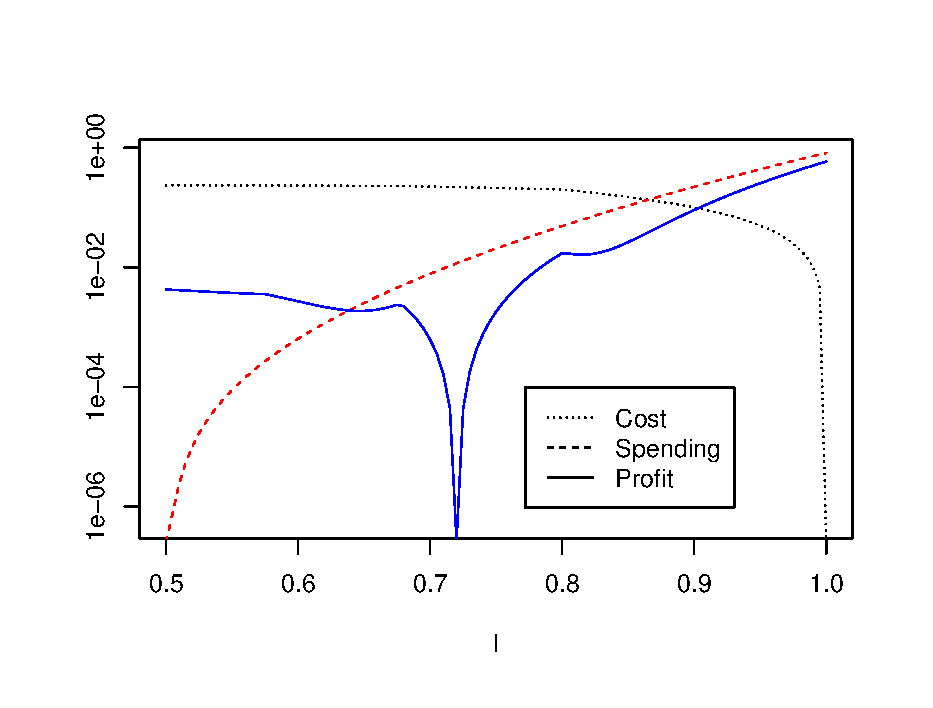
\includegraphics[trim=0mm 5mm 5mm 15mm, clip, width=\linewidth]{figures/suboptimality.eps}
    \caption{Suboptimality of Cost, Spending and Profit over $l$ when $n = 10, b = 0.2, c = 0.1$}\label{fig:suboptimality}
\end{figure}

As you can see from figure \ref{fig:suboptimality}, the cost isn't unimodal over $l$ and it's quite wierd.
Thus in later experiments, we are just going to brute forcely search over all possible $l$ from $0.5$ to $1$,
with a search increment of $0.01$.

\subsection{Experiments}

Now we are going to compare profit of different mechanisms in general settings.
To keep it simple, we still use a uniform valuation distribution for all
experiments.  As theorem \ref{theorem:equivalence} shows, the profit is simply
spending minus cost where spending is solely determined by $l$. In fact, the
total spending won't be very sensitive to this $l$ when $n$ is large (except
that $l$ is very close to $1$) and we will see this in later comparisons. Thus
most experimental comparisons that we have done for cost in section
\ref{sec:eff_experiment} would also give us a lot information for profit
comparison. As a result, we will compare mechanisms very different from those
in section \ref{sec:eff_experiment}. Specifically, we won't be interested in
$k$-MVA where $k$ is very limited. Instead, we are going to compare how $l$
is going to affect the profit and how much profit we lose if we ignore the cost.

If we ignore the cost, Myerson has already proved that a singleshot Vickrey
auction with reserve price $0.5$ would be optimal for uniform i.i.d. bidders.
Thus we will compare this singleshot mechanism, as well as its variants, the
singleshot Vickrey auction with $0$ reserve price. But be aware of that reserve
price isn't equivalent with low value $l$  when cost exists. To make it more fair,
we add one more singleshot Vickrey auction whose reserve is set to be optimal
among all singleshot Vickrey auctions (i.e. we optimize $l$ for this particular
singleshot mechanism).
One may also suspect whether it's good enough to set low value $l$ to be $0.5$
in such singleshot Vickrey auction, since it will bring us maximal total
spending. The answer is no, because its bidding cost is $0.5 n \times c$, which
grows way too large when $n$ is large.

\begin{figure}
\centering
  \subfigure[profit]{
    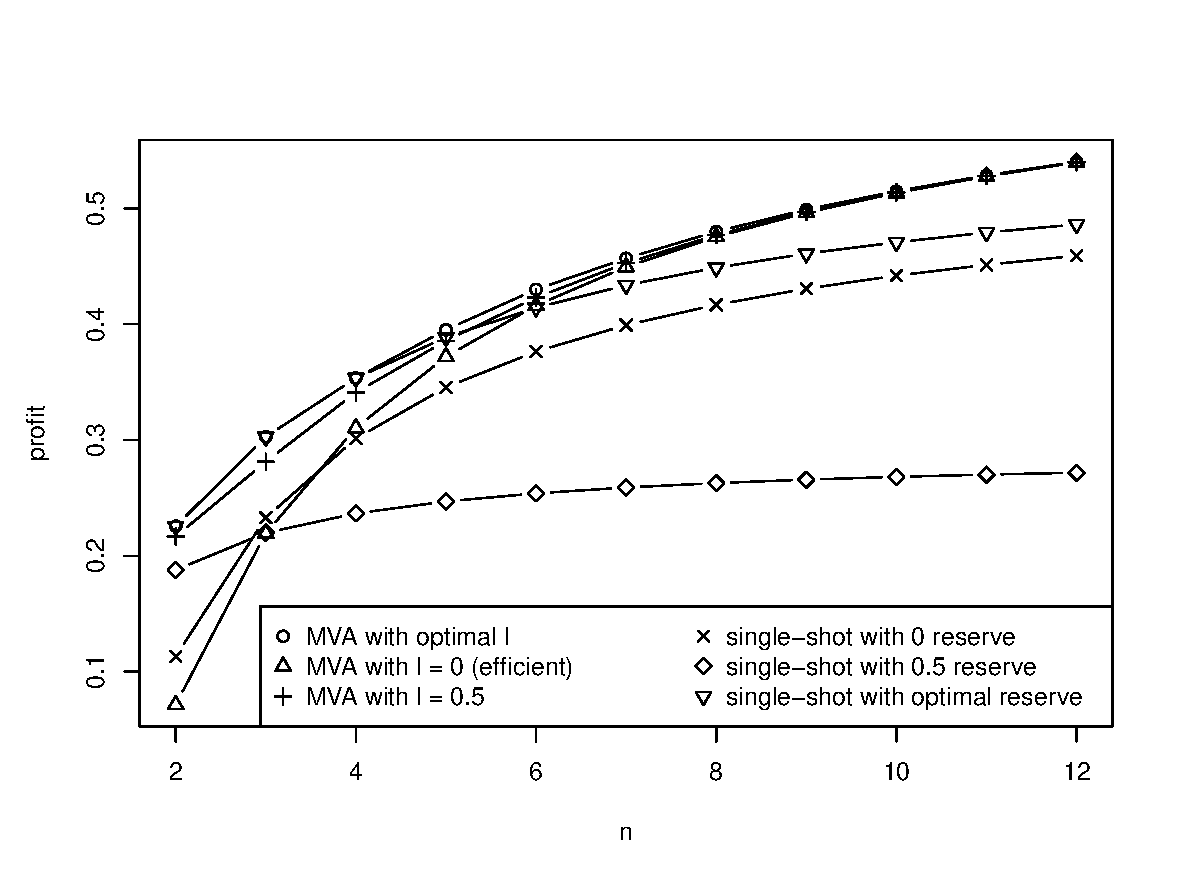
\includegraphics[trim=0mm 5mm 5mm 15mm, clip, width=\linewidth]{figures/profit_.1.eps}
    \label{fig:general_profit}
  }
  \subfigure[low value]{
    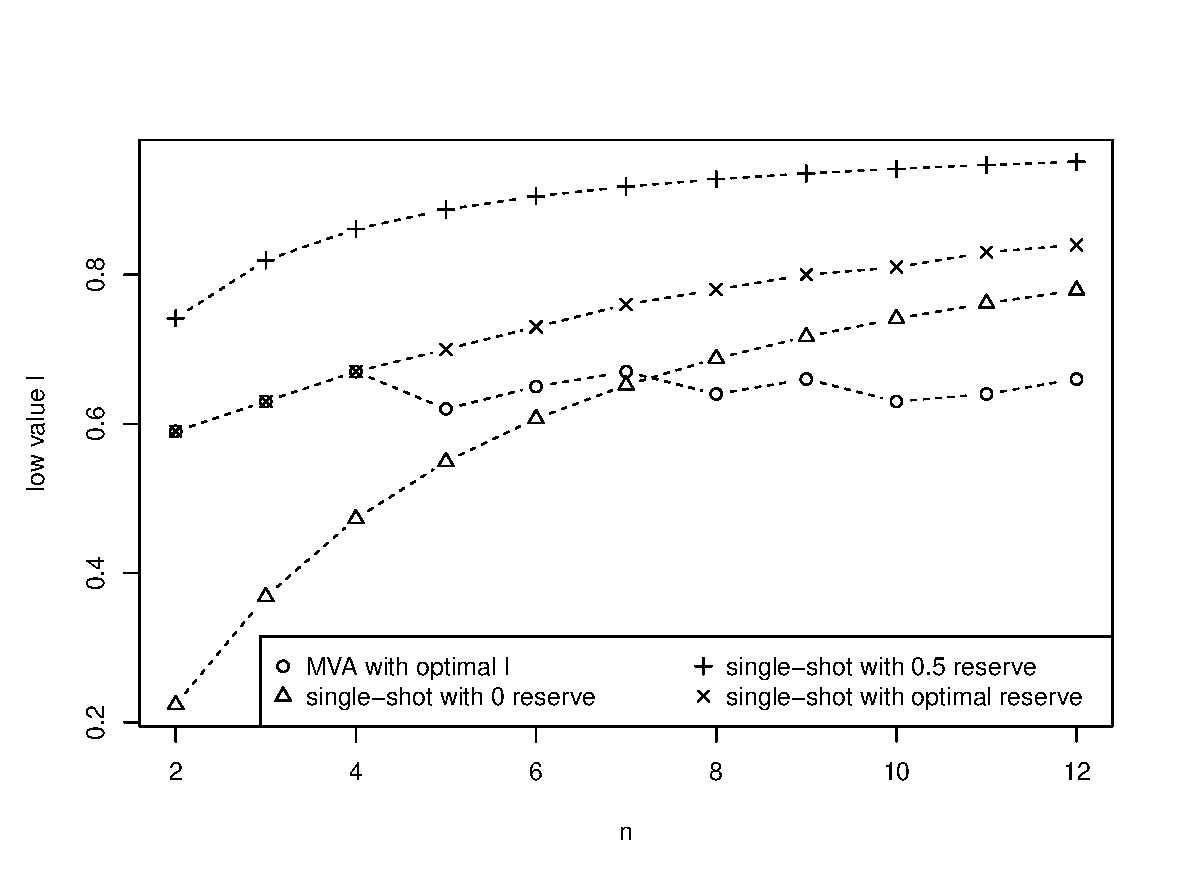
\includegraphics[trim=0mm 5mm 5mm 15mm, clip, width=\linewidth]{figures/l_.1.eps}
    \label{fig:general_l}
  }
  \caption{Compare profit and corresponding low value $l$ over $n$. The
  broadcast cost $b = 0.1$. Bidding cost for seller and buyer are $\beta_1 =
  \beta_2 = 0.05$ (thus $c = \beta_1+\beta_2 = 0.1$)}\label{fig:general}
\end{figure}

The experimental result is shown in figure \ref{fig:general}. As shown in
profit comparison figure \ref{fig:general_profit}, the profit of optimal $l$,
$l = 0$ and $l = 0.5$ become close very quickly when $n$ grows and they are
almost identical for $n \geq 8$ in this experiment setting. Thus choosing $l$
won't be a critical issue for large $n$. However, if we use singleshot
mechanism (which is optimal if cost doesn't exist), the gap is significant.
This is because the bidding cost will drive low value $l$ very
close to $1$ thus lower the total spending significantly. For example, even if
we set reserve price to $0$, when $n = 10$, $l$ will be between $0.6$ to $0.8$.
The optimal reserve price $0.5$ becomes the worst as its $l$ is too high. 
Even if we adapt our reserve price to optimal one, the singleshot mechanism is
still not so good because it can't balance the total spending and bidding cost,
i.e. it either makes $l$ close to $1$ to lose a lot total spending, or makes
$l$ close to $0.5$ to cause a big bidding cost.
